% Document packages / layout
\documentclass[
    pdf,
    11pt,
    xcolor={svgnames},
    %hyperref={colorlinks, citecolor=Cyan, linkcolor=Cyan, urlcolor=Cyan}
  ]{beamer}
%\usetheme{Copenhagen}
\usetheme{Madrid}
\usecolortheme{beaver}
\usepackage{color}

\usepackage[style=alphabetic]{biblatex}
\addbibresource{citations.bib}

% Remove navigation controls
\setbeamertemplate{navigation symbols}{}

% Un-numbered footnote
\newcommand\blfootnote[1]{%
  \begingroup
  \renewcommand\thefootnote{}\footnote{\scriptsize #1}%
  \addtocounter{footnote}{-1}%
  \endgroup
}

% Figure Packages
\usepackage{float}
\usepackage{subcaption}

% Math Packages
\usepackage{amsmath,amsthm,amssymb,mathrsfs,bm}
\usepackage{commath}
\usepackage{physics}

% Quality of Life Packages
\usepackage{enumerate}
\usepackage{siunitx} %\sisetup{inter-unit-product =$\cdot$}
\usepackage{multicol}
\usepackage{wrapfig}
\usepackage{graphicx}

%\newtheorem*{definition}{Definition}

% Creates section subdivider at beginning of each section.
\AtBeginSection[]
{
  \begin{frame}
    \frametitle{Table of Contents}
    \tableofcontents[currentsection]
  \end{frame}
}
 
\title[WBSG for Random Scalar Hyperbolic Laws]{%
  A Well-Balanced Stochastic Galerkin for Scalar Hyperbolic Laws with Random Forcing.
}
\author[Chowdhary, Shedlock]{%
  Andrew Shedlock and Abhijit Chowdhary
}
\institute[NCSU]{
  Department of Mathematics \\
  North Carolina State University
}
\date[MA788 NCSU]{\today}

\begin{document}

\frame{ \titlepage }

\begin{frame}
\begin{figure}
\centering
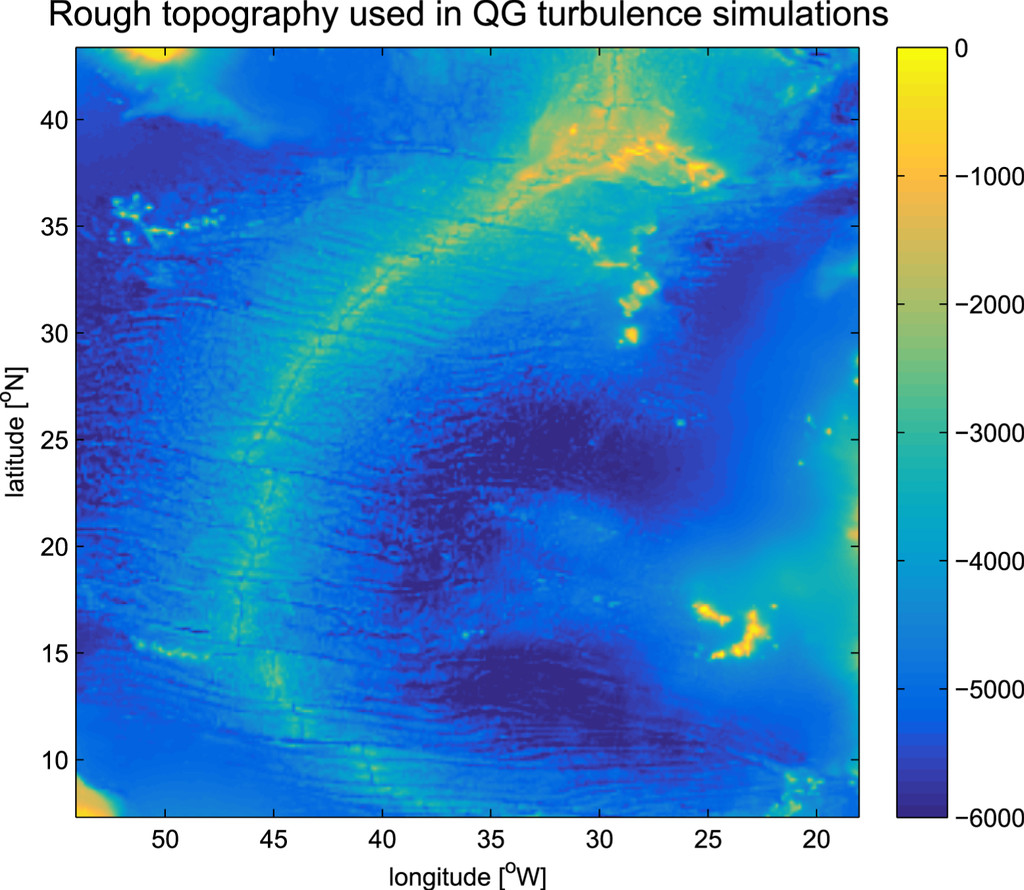
\includegraphics[width=0.70\textwidth]{slides/bottom_topography.jpg}
\end{figure}
\blfootnote{\fullcite{Trossman2017}}
\end{frame}

\begin{frame}
    \frametitle{Difficulties in real-world simulation}
    \begin{columns}
    \begin{column}{0.5\textwidth}
    If the given bottom topography given was our source term, we would have:
    \vspace{-1em}
    \begin{itemize}
        \item Uncertainty in measurement
        \item Low regularity
    \end{itemize}
    The former can have a non-negligible effect on simulation and the latter can pose difficulties in capturing the true steady state solution.
    \end{column}
    \begin{column}{0.5\textwidth}
        \begin{figure}
        \centering
        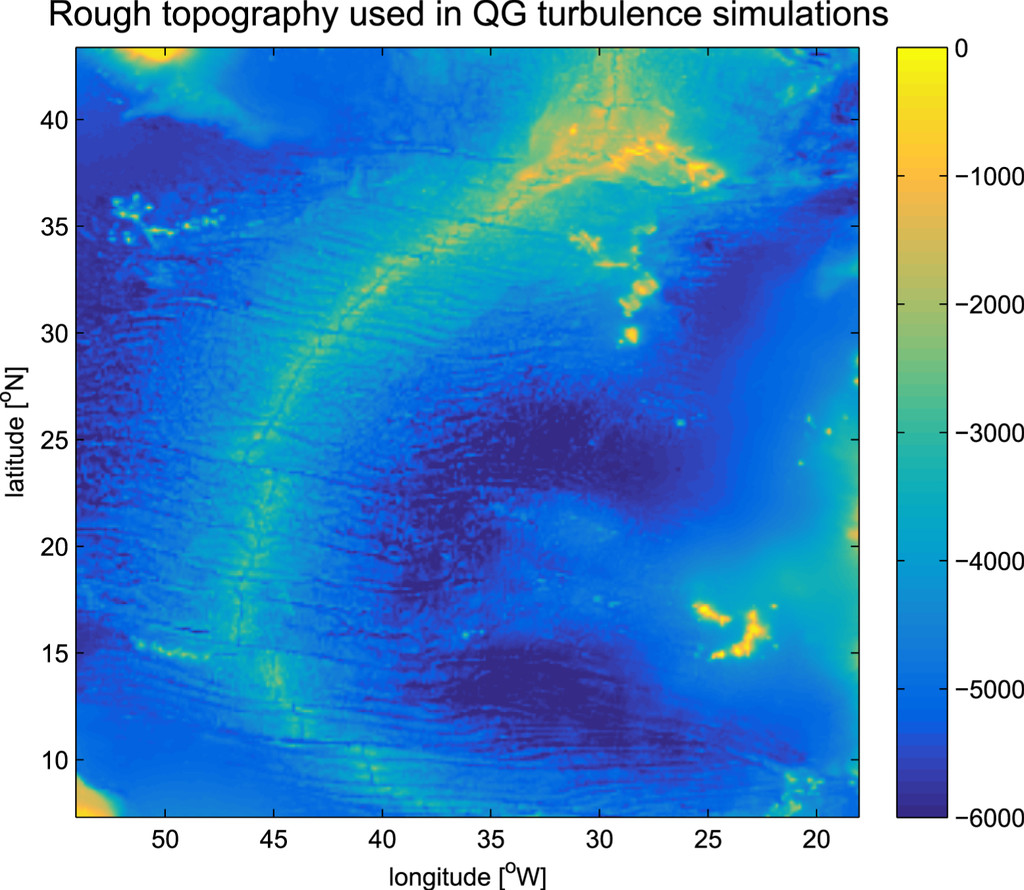
\includegraphics[width=\textwidth]{slides/bottom_topography.jpg}
        \end{figure}
    \end{column}
    \end{columns}
    {\bf Idea:} Combine previous ideas for stochastic Galerkin via generalized polynomial chaos and well-balanced interface methods.
    \blfootnote{\fullcite{Jin2015}}
\end{frame}

%%%%%%%%%%%%%%%%%%%%%%%%%%%%%%%%%%%%%%%%%%%%%%%%%%%%%%%%%%%%%%%%%%%%%%%%%%%%%%%
%%% Preliminaries
%%%%%%%%%%%%%%%%%%%%%%%%%%%%%%%%%%%%%%%%%%%%%%%%%%%%%%%%%%%%%%%%%%%%%%%%%%%%%%%
\section{Preliminaries}

\begin{frame}{Model Problem}
    Given the scalar conservation law with source term:
    \begin{equation} \label{eq:model}
        \partial_t u + \partial_x f(u) = -b'(x) q(u).
    \end{equation}
    we have the steady-state equation
    \begin{equation} \label{eq:model_ss}
         \partial_x f(u) + -b'(x) q(u) = 0.
    \end{equation}
    which, supposing a smooth solution, can be written into:
    \begin{equation} \label{eq:ss_condition}
        \begin{cases}
            D(u(z)) + b(x) = {\rm constant}. \\
            D(u) = \int_0^u \frac{f'(u)}{q(u)} \dd{s}
        \end{cases}
    \end{equation}
    which we call the steady-state condition.
\end{frame}

\subsection{A Well-Balanced Deterministic Scheme}
\begin{frame}{A Well-Balanced Numerical Scheme}
    \begin{definition}
        A numerical scheme is called well-balanced (WB) if it can preserve the steady-state condition \eqref{eq:ss_condition} either exactly, or formally with at least second order accuracy.
    \end{definition}
\end{frame}

\begin{frame}{FVM Framework}
    Consider the uniform discretization:
    \begin{itemize}
        \item $(x_{j+1/2})_{j=1}^{N_x}$ with $\Delta x = x_{j+1/2}-x_{j-1/2}$;
        \item $(t_n)_{n=1}^{N_t}$ with $\Delta t = t^n - t^{n-1}$.
    \end{itemize}
    \pause
    Define:
    \begin{equation*}
        u_j^n = \frac{1}{\Delta x} \int_{x_{j-1/2}}^{x_{j+1/2}} u(x,t^n) \dd{x}
    \end{equation*}
    \pause
    and construct the semi-discrete interface method proposed in \cite{Jin2001}:
    \begin{equation}
        \partial_t u_j + \frac{f_{j+1/2} - f_{j-1/2}}{\Delta x} = - \frac{b_{j+1/2} - b_{j-1/2}}{\Delta x} \frac{q_{j+1/2} + q_{j-1/2}}{2}
    \end{equation}
    \pause
    or if $D(u)$ is monotone
    \begin{equation} \label{eq:deterministic_scheme}
        \partial_t u_j + \frac{f_{j+1/2} - f_{j-1/2}}{\Delta x} = - \frac{b_{j+1/2} - b_{j-1/2}}{\Delta x} \frac{f_{j+1/2} + f_{j-1/2}}{D_{j+1/2}-D_{j-1/2}}
    \end{equation}
\end{frame}

% Pause is broken in align 
% https://tex.stackexchange.com/questions/6348/problem-with-beamers-pause-in-alignments
\begin{frame}
    Hence, considering the steady state solution:
    \begin{align*}
        & 
        \frac{f_{j+1/2} - f_{j-1/2}}{\Delta x} + \frac{b_{j+1/2} - b_{j-1/2}}{\Delta x} \frac{f_{j+1/2} + f_{j-1/2}}{D_{j+1/2}-D_{j-1/2}} = 0
    \end{align*}
\end{frame}
\begin{frame}
    Hence, considering the steady state solution:
    \begin{align*}
        & 
        \frac{f_{j+1/2} - f_{j-1/2}}{\Delta x} + \frac{b_{j+1/2} - b_{j-1/2}}{\Delta x} \frac{f_{j+1/2} + f_{j-1/2}}{D_{j+1/2}-D_{j-1/2}} = 0 \\
        \implies\ 
        &
        D_{j+1/2} - D_{j-1/2} + b_{j+1/2} - b_{j-1/2} = 0
    \end{align*}
\end{frame}
\begin{frame}
    Hence, considering the steady state solution:
    \begin{align*}
        & 
        \frac{f_{j+1/2} - f_{j-1/2}}{\Delta x} + \frac{b_{j+1/2} - b_{j-1/2}}{\Delta x} \frac{f_{j+1/2} + f_{j-1/2}}{D_{j+1/2}-D_{j-1/2}} = 0 \\
        \implies\ 
        &
        D_{j+1/2} - D_{j-1/2} + b_{j+1/2} - b_{j-1/2} = 0 \\
        \implies\ 
        &
        D_{j+1/2} + b_{j+1/2} = {\rm constant}
    \end{align*}
    Thus, the steady state condition \eqref{eq:ss_condition} is preserved exactly at the cell interface.
\end{frame}

\subsection{gPC approximation and stochastic Galerkin}
\begin{frame}{Introduction to stochastic Galerkin via gPC}
    Consider a general SDE with random inputs:
    \begin{equation} \label{eq:SDE}
        \partial_t u = \mathcal{L}(t,x,u,z;b(x,z))
    \end{equation}
    where, for convenience, let $z \in I_z \subset \mathbb{R}$ parameterize the random input.
    
    \pause
    
    Let $\mathbb{P}_N$ denote the space of orthonormal polynomials of degree up to $N$. Call
    \begin{align*}
        u(x,t,z) &= u_N(x,t,z) = \sum_{m=1}^M \hat{u}_m(t,x) \Phi_m(z) \\
        b(x,z) &= u_N(x,z) = \sum_{m=1}^M \hat{b}_m(t,x) \Phi_m(z) 
    \end{align*}
    the gPC expansions of the associated variables, where $(\Phi_m)_{m=1}^M \subset \mathbb{P}_N$ is typically chosen based on the distribution of $z$ in order to guarantee faster coefficient convergence.
\end{frame}


%%%%%%%%%%%%%%%%%%%%%%%%%%%%%%%%%%%%%%%%%%%%%%%%%%%%%%%%%%%%%%%%%%%%%%%%%%%%%%%
%%% Stochastic WB scheme for Burgers
%%%%%%%%%%%%%%%%%%%%%%%%%%%%%%%%%%%%%%%%%%%%%%%%%%%%%%%%%%%%%%%%%%%%%%%%%%%%%%%
\section{A WBSG scheme for Burgers' equation}

\begin{frame}{Burgers' equation}
    Consider Burgers' equation with a random source term
    \begin{equation}
        \partial_t u + \partial_x \left( \frac{u^2}{2} \right) = -b'(x,z) u
    \end{equation}
    \pause
    We apply the interface method to find
    \begin{equation} \label{eq:burgers_inteface}
        \partial_t u_j + \frac{u_j^2 - u_{j-1}^2}{2 \Delta x} = -\frac{b_j - b_{j-1}}{\Delta x} \frac{u_j + u_{j-1}}{2}
    \end{equation}
    where we've applied an upwind flux assuming $u > 0$ for brevity.
\end{frame}

\begin{frame}{sWB Burgers}
    Replacing $u_j$ and $b_j$ with their gPC approximation and taking an expectation of \eqref{eq:burgers_inteface}, we find:
    \begin{multline*}
        \mathbb{E}\left[
            \left(
                \pdv{}{t} u_{N,j} + \frac{u_{N,j}^2-u_{N,j-1}^2}{2\Delta x}
            \right) \Phi_m(z)
        \right] \\
        = -\mathbb{E} \left[
            \frac{b_{N,j} - b_{N,j-1}}{\Delta x} \frac{u_{N,j} - u_{N,j-1}}{2} \Phi_m(z)
        \right]
    \end{multline*}
    \pause
    Finally, substitute in the gPC expansions and and use orthonormality to find:
\end{frame}

\begin{frame}{sWB Burgers Full Scheme}
   \begin{equation}
       \partial_t \hat{\vb{u}}_j + \frac{\vb{A}_j \hat{\vb{u}}_j - \vb{A}_{j-1} \hat{\vb{u}}_{j-1}}{2\Delta x} = -\frac{(\vb{B}_j - \vb{B}_{j-1})(\hat{\vb{u}}_j + \hat{\vb{u}}_{j-1})}{2\Delta x}
   \end{equation} 
   where:
   \begin{equation*}
       \hat{\vb{u}} = (\hat{u}_1, \dots, \hat{u}_M)^\mathrm{T}
       \qquad
       \hat{\vb{b}} = (\hat{b}_1, \dots, \hat{b}_M)^\mathrm{T}
   \end{equation*}
   \begin{align*}
       [\vb{A}_j]_{mn} &= \mathbb{E}[u_{N,j} \Phi_m \Phi_n] = \sum_{k=1}^M \hat{u}_{k,j} e_{kmn} \\
       [\vb{B}_j]_{mn} &= \mathbb{E}[b_{N,j} \Phi_m \Phi_n] = \sum_{k=1}^M \hat{b}_{k,j} e_{kmn}
   \end{align*}
   with $e_{kmn} = \mathbb{E}[\Phi_k \Phi_m \Phi_n]$.
\end{frame}

\begin{frame}
    Our scheme:
   \begin{equation*}
       \partial_t \hat{\vb{u}}_j + \frac{\vb{A}_j \hat{\vb{u}}_j - \vb{A}_{j-1} \hat{\vb{u}}_{j-1}}{2\Delta x} = -\frac{(\vb{B}_j - \vb{B}_{j-1})(\hat{\vb{u}}_j + \hat{\vb{u}}_{j-1})}{2\Delta x}
   \end{equation*} 
   reduces to
   \begin{equation*}
       \frac{\vb{A}_j \hat{\vb{u}}_j - \vb{A}_{j-1} \hat{\vb{u}}_{j-1}}{2\Delta x} + \frac{(\vb{B}_j - \vb{B}_{j-1})(\hat{\vb{u}}_j + \hat{\vb{u}}_{j-1})}{2\Delta x} = 0
   \end{equation*} 
   in the steady state case. The proof that this is WB follows from the earlier one in the deterministic case.
\end{frame}

\begin{frame}{An alternative flux}
    Likewise, with flux $f(u) = u^4 / 4$ we can derive a similar method:
   \begin{equation}
       \partial_t \hat{\vb{u}}_j + \frac{\vb{S}_j \hat{\vb{u}}_j - \vb{S}_{j-1} \hat{\vb{u}}_{j-1}}{4\Delta x} = -\frac{(\vb{B}_j - \vb{B}_{j-1})(\hat{\vb{u}}_j + \hat{\vb{u}}_{j-1})}{2\Delta x}
   \end{equation} 
   where:
   \begin{equation*}
       \hat{\vb{u}} = (\hat{u}_1, \dots, \hat{u}_M)^\mathrm{T}
       \qquad
       \hat{\vb{b}} = (\hat{b}_1, \dots, \hat{b}_M)^\mathrm{T}
   \end{equation*}
   \begin{align*}
       [\vb{S}_j]_{mn} &= \mathbb{E}[u_{N,j}^3 \Phi_m \Phi_n]  = \sum_{p,q,r}^M \hat{u}_{p,j} \hat{u}_{q,j} \hat{u}_{r,j} d_{pqrmn}\\
       [\vb{B}_j]_{mn} &= \mathbb{E}[b_{N,j} \Phi_m \Phi_n] = \sum_{k=1}^M \hat{b}_{k,j} e_{kmn}
   \end{align*}
   with $e_{kmn} = \mathbb{E}[\Phi_k \Phi_m \Phi_n]$ and $d_{pqrmn} = \mathbb{E}[\Phi_p \Phi_q \Phi_r \Phi_m \Phi_n]$. (Agony)
\end{frame}

%%%%%%%%%%%%%%%%%%%%%%%%%%%%%%%%%%%%%%%%%%%%%%%%%%%%%%%%%%%%%%%%%%%%%%%%%%%%%%%
%%% Numerical Considerations
%%%%%%%%%%%%%%%%%%%%%%%%%%%%%%%%%%%%%%%%%%%%%%%%%%%%%%%%%%%%%%%%%%%%%%%%%%%%%%%
\section{Numerical Considerations}
\begin{frame}{Numerical Considerations}
   \begin{equation*}
       \partial_t \hat{\vb{u}}_j + \frac{\vb{A}_j \hat{\vb{u}}_j - \vb{A}_{j-1} \hat{\vb{u}}_{j-1}}{2\Delta x} = -\frac{(\vb{B}_j - \vb{B}_{j-1})(\hat{\vb{u}}_j + \hat{\vb{u}}_{j-1})}{2\Delta x}
   \end{equation*} 
   There are a couple of points to note regarding this scheme:
   \begin{itemize}[<+->]
       \item $\hat{u}$ has $N_x \times M$ entries;
       \item $\vb{B}$ is constant in time $\implies$ can be computed before time evolution
       \item $\vb{A}$ depends on time $\implies$ must be computed per time step.
       \item $\vb{A}_j$ and $\vb{B}_j$ are symmetric.
   \end{itemize}
   Based on profiling, the computation of $\vb{A}$ dominates runtime.
\end{frame}

%%%%%%%%%%%%%%%%%%%%%%%%%%%%%%%%%%%%%%%%%%%%%%%%%%%%%%%%%%%%%%%%%%%%%%%%%%%%%%%
%%% Results
%%%%%%%%%%%%%%%%%%%%%%%%%%%%%%%%%%%%%%%%%%%%%%%%%%%%%%%%%%%%%%%%%%%%%%%%%%%%%%%
\section{Results}
\begin{frame}{Mean: Why well-balanced matters}
    \begin{figure}
    \centering
    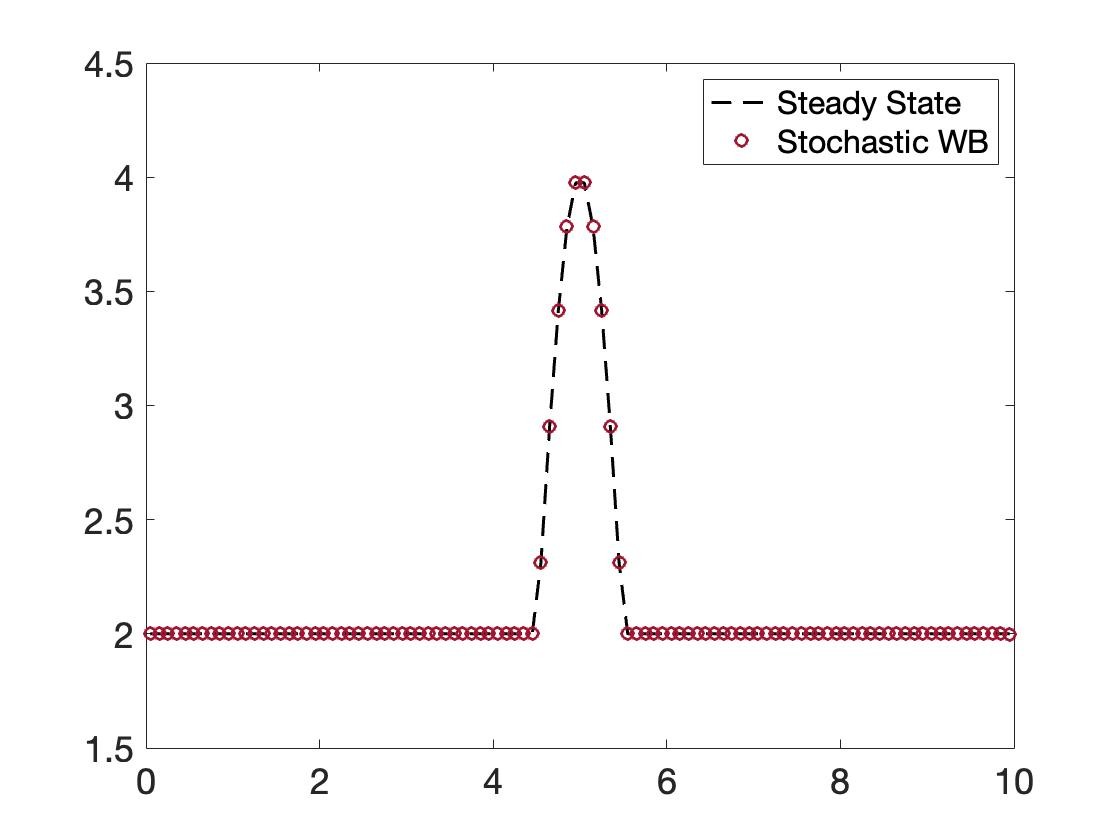
\includegraphics[width=0.85\textwidth]{./Figures/burgers_wb_mean}
    \end{figure}
\end{frame}
\begin{frame}{Mean: Why well-balanced matters}
    \begin{figure}
    \centering
    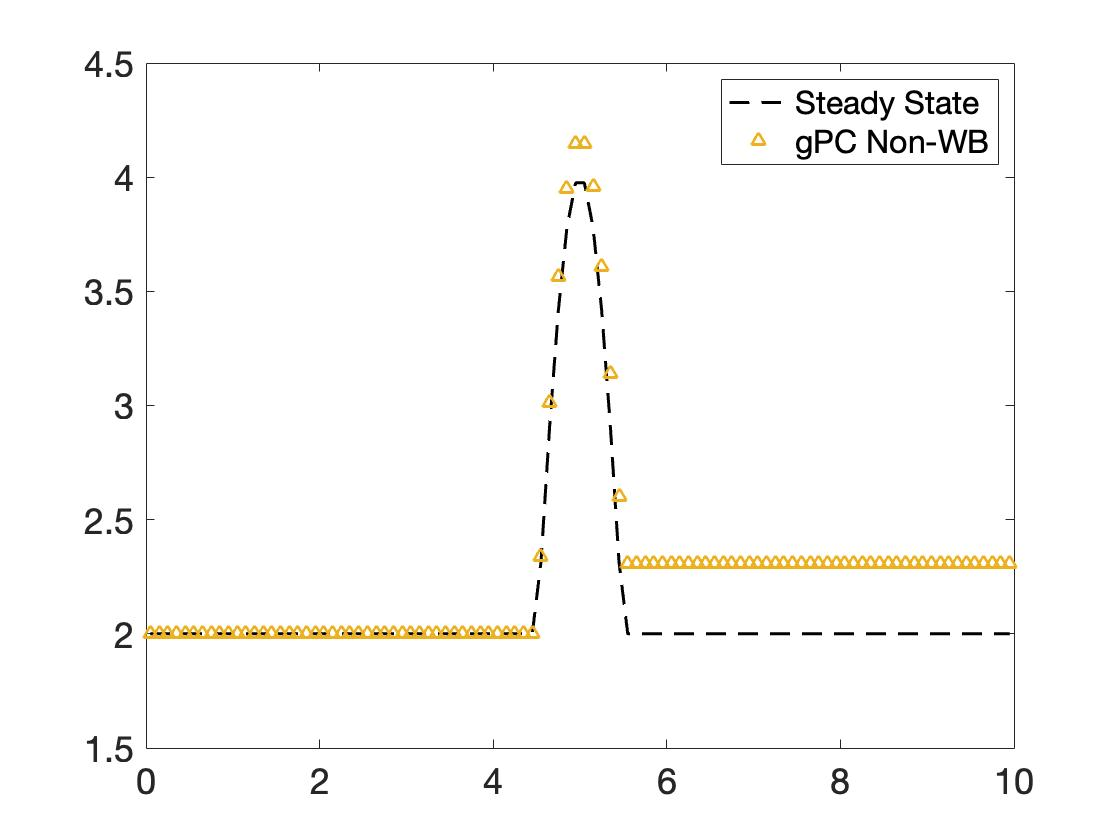
\includegraphics[width=0.85\textwidth]{./Figures/burgers_non_mean}
    \end{figure}
\end{frame}

\begin{frame}{Standard Deviation: Why well-balanced matters}
    \begin{figure}
    \centering
    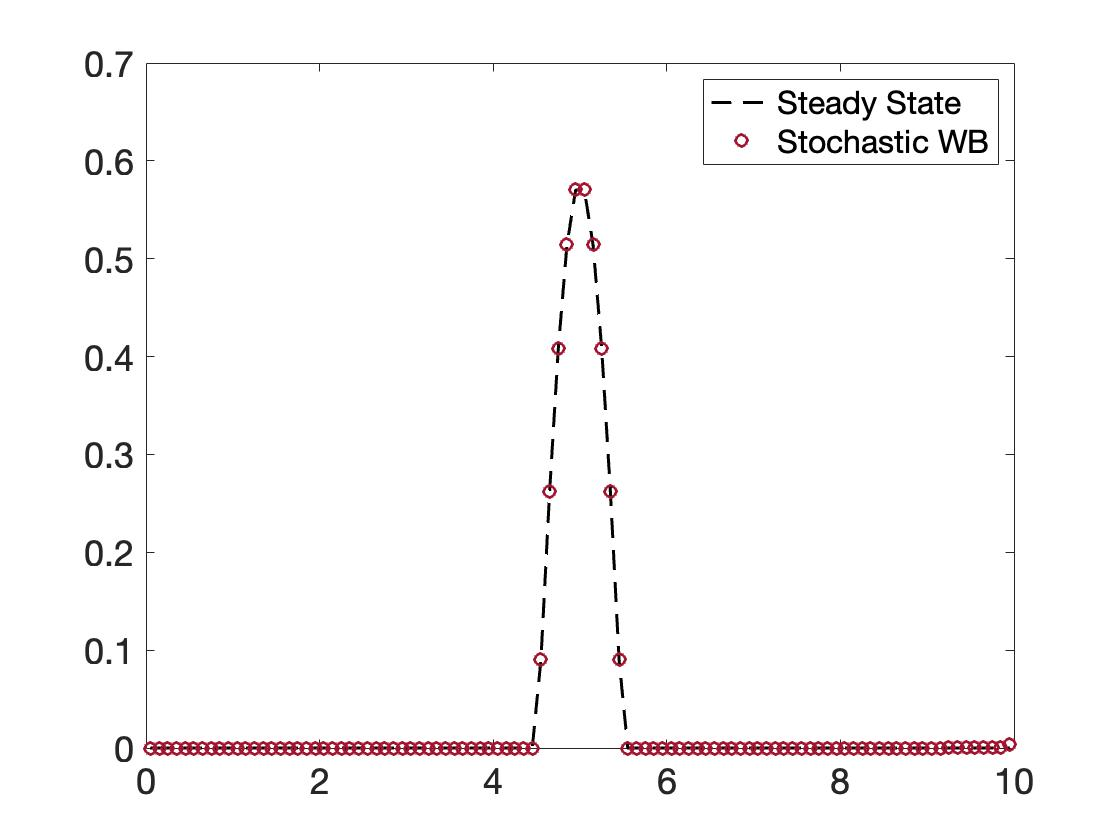
\includegraphics[width=0.85\textwidth]{./Figures/burgers_wb_sd}
    \end{figure}
\end{frame}
\begin{frame}{Standard Deviation: Why well-balanced matters}
    \begin{figure}
    \centering
    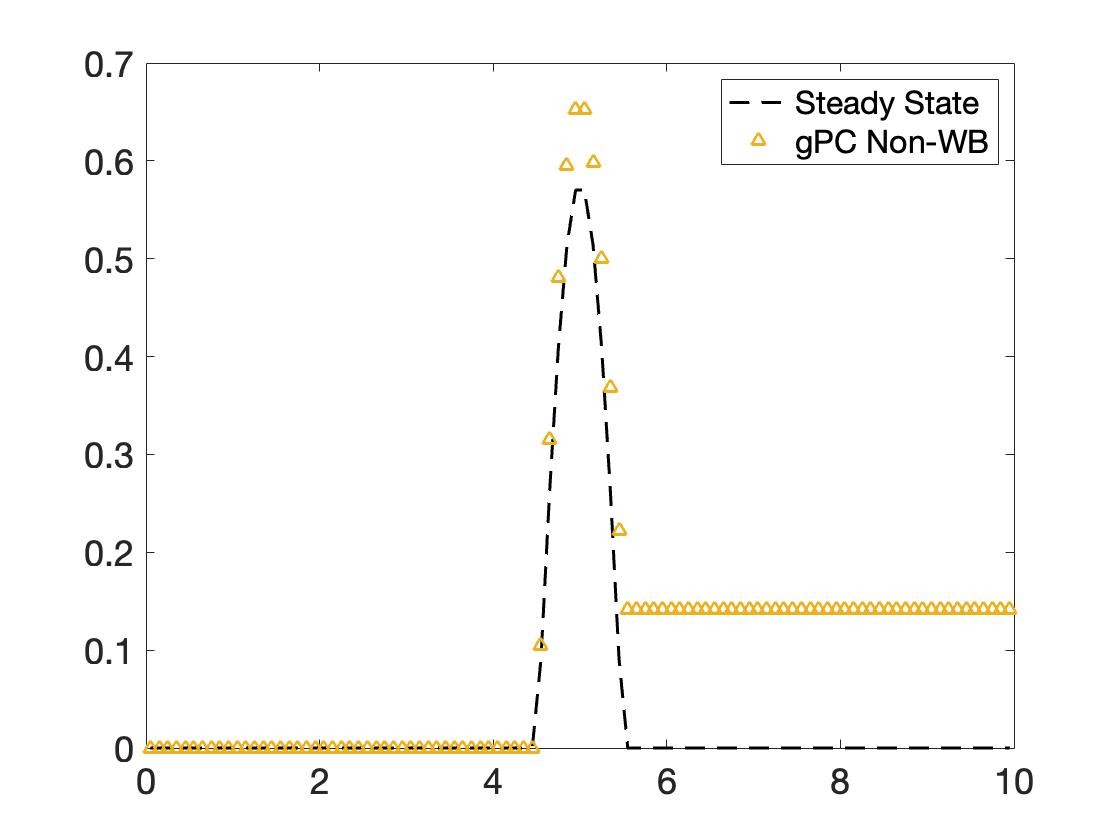
\includegraphics[width=0.85\textwidth]{./Figures/burgers_non_sd}
    \end{figure}
\end{frame}

\begin{frame}{Mean: Discontinuous bottom topography}
    \begin{figure}
    \centering
    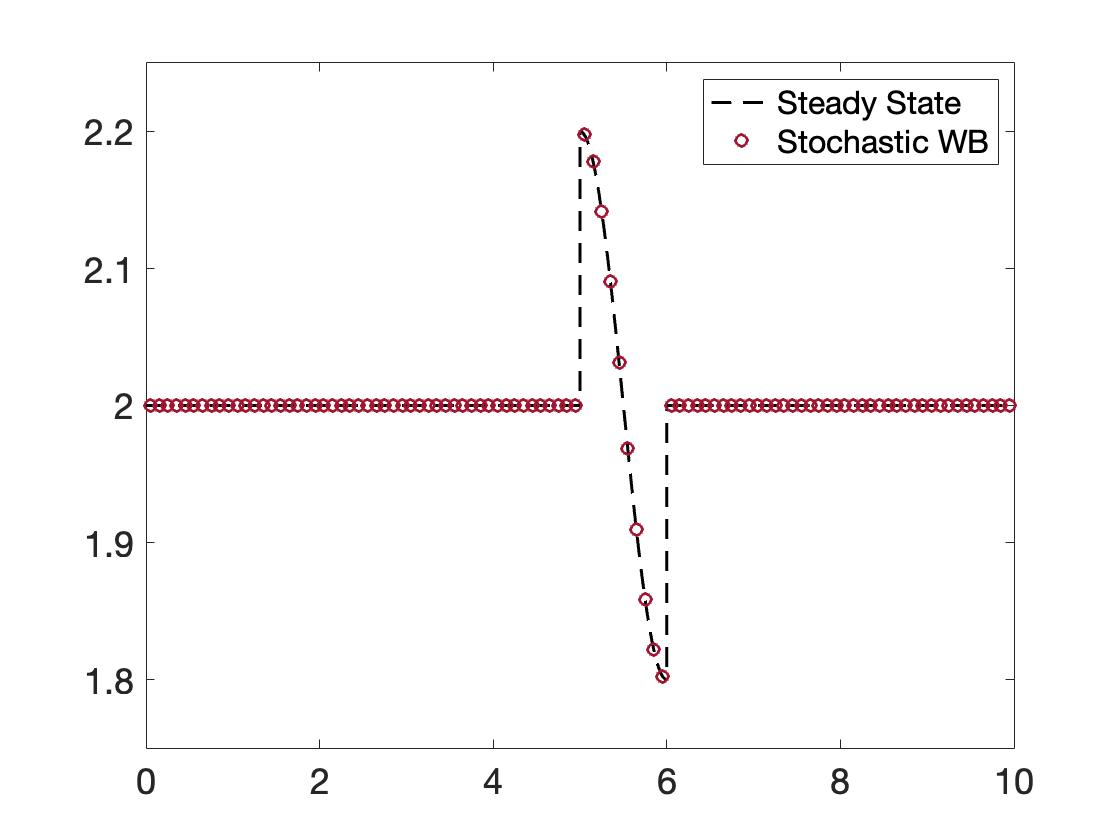
\includegraphics[width=0.85\textwidth]{./Figures/burgers_dis_wb_mean}
    \end{figure}
\end{frame}
\begin{frame}{Mean: Discontinuous bottom topography}
    \begin{figure}
    \centering
    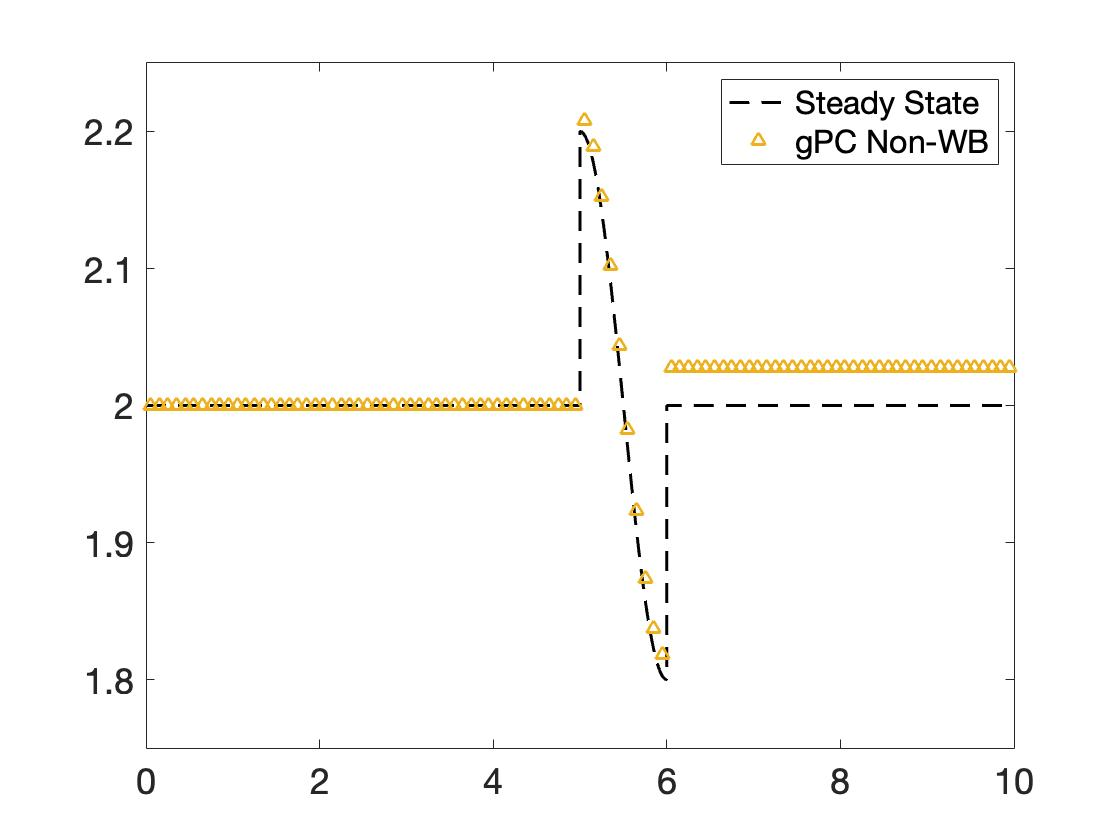
\includegraphics[width=0.85\textwidth]{./Figures/burgers_dis_non_mean}
    \end{figure}
\end{frame}

\begin{frame}{Standard Deviation: Discontinuous bottom topography}
    \begin{figure}
    \centering
    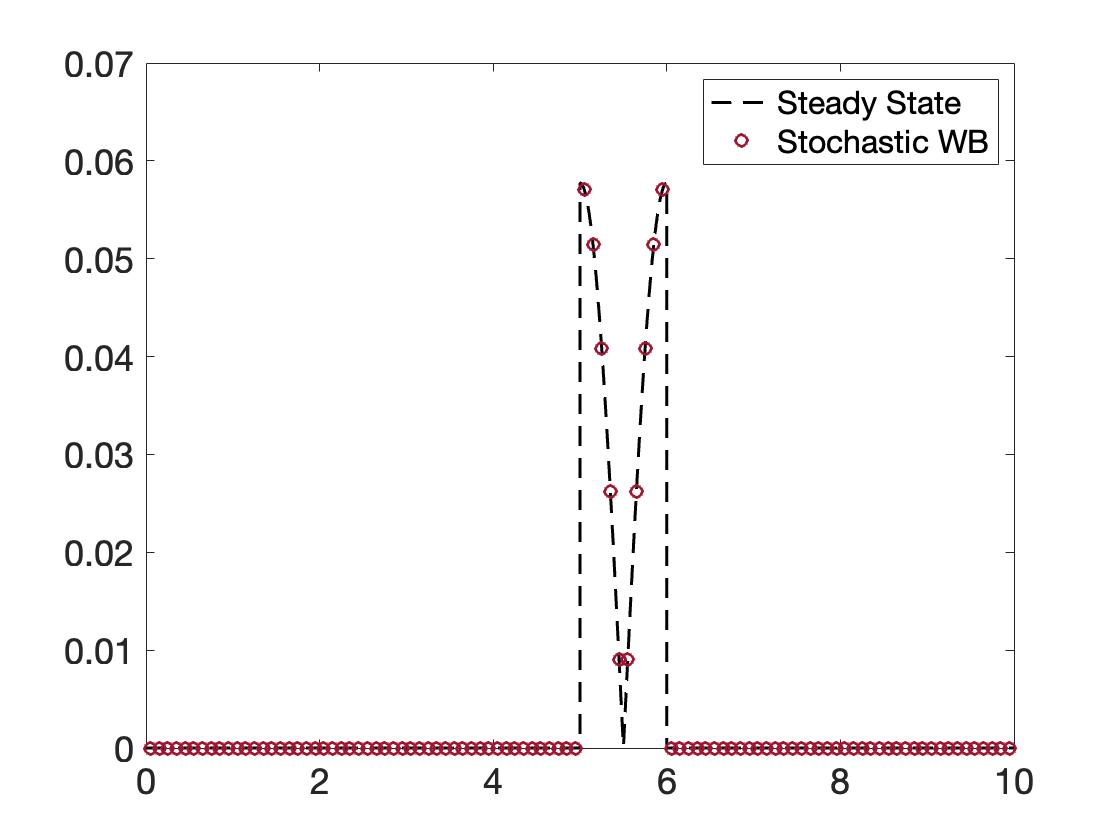
\includegraphics[width=0.85\textwidth]{./Figures/burgers_dis_wb_sd}
    \end{figure}
\end{frame}
\begin{frame}{Standard Deviation: Discontinuous bottom topography}
    \begin{figure}
    \centering
    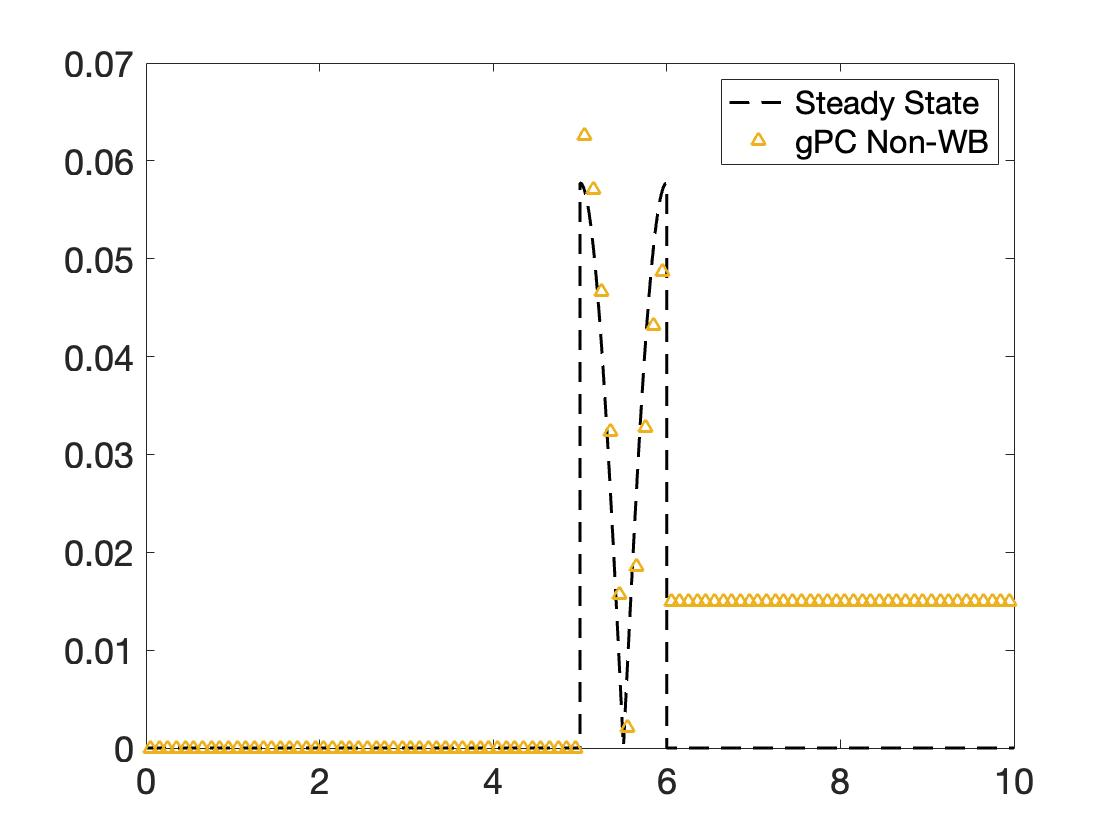
\includegraphics[width=0.85\textwidth]{./Figures/burgers_dis_non_sd}
    \end{figure}
\end{frame}

%%%%%%%%%%%%%%%%%%%%%%%%%%%%%%%%%%%%%%%%%%%%%%%%%%%%%%%%%%%%%%%%%%%%%%%%%%%%%%%
%%% Discussion and Future Work
%%%%%%%%%%%%%%%%%%%%%%%%%%%%%%%%%%%%%%%%%%%%%%%%%%%%%%%%%%%%%%%%%%%%%%%%%%%%%%%
\section{Discussion and Improvements}

%%%%%%%%%%%%%%%%%%%%%%%%%%%%%%%%%%%%%%%%%%%%%%%%%%%%%%%%%%%%%%%%%%%%%%%%%%%%%%%
%%% References
%%%%%%%%%%%%%%%%%%%%%%%%%%%%%%%%%%%%%%%%%%%%%%%%%%%%%%%%%%%%%%%%%%%%%%%%%%%%%%%
\begin{frame}{References}
\printbibliography
\end{frame}

\end{document}